%!TEX program = xelatex
% hard_way.tex
\documentclass[UTF8, a4paper, zihao = 5]{ctexbook}

\title{笨办法学 \LaTeX}
\author{Liam Huang}
\date{\today}

\usepackage{amsmath}
\usepackage{hyperref}
\usepackage[normalem]{ulem}
\usepackage{enumitem}
\setlist{nosep}
\usepackage{caption}
% settings for caption.sty
\DeclareCaptionFormat{mylst}{\hrule#1#2#3}
\captionsetup[lstlisting]{
  format          = mylst,
  labelfont       = bf,
  singlelinecheck = off,
  labelsep        = space
}
\endinput

\usepackage{graphicx}
\graphicspath{{./pic/}}
\usepackage[usenames, dvipsnames]{xcolor}
\usepackage{listings}
% settings for listings.sty
\renewcommand{\lstlistingname}{代码清单}
\lstdefinestyle{lfonts}{
  basicstyle   = \footnotesize\ttfamily,
  stringstyle  = \color{purple},
  keywordstyle = \color{blue!60!black}\bfseries,
  commentstyle = \color{olive}\scshape,
}
\lstdefinestyle{lnumbers}{
  numbers     = left,
  numberstyle = \tiny,
  numbersep   = 1em,
  firstnumber = 1,
  stepnumber  = 1,
}
\lstdefinestyle{llayout}{
  breaklines       = true,
  tabsize          = 2,
  columns          = flexible,
}
\lstdefinestyle{lgeometry}{
  xleftmargin      = 20pt,
  xrightmargin     = 0pt,
  frame            = tb,
  framesep         = \fboxsep,
  framexleftmargin = 20pt,
}
\lstdefinestyle{lgeneral}{
  style = lfonts,
  style = lnumbers,
  style = llayout,
  style = lgeometry,
}
\def\beginlstdelim#1#2#3{%
  \def\endlstdelim{#2\egroup}%
  \ttfamily#1\bgroup\color{#3}\aftergroup\endlstdelim}
\lstdefinestyle{ldelims}{
  moredelim = **[is][\beginlstdelim{\$}{\$}{orange}]{\$}{\$},
  moredelim = **[is][\beginlstdelim{\{}{\}}{ForestGreen}]{\{}{\}},
  moredelim = **[is][\beginlstdelim{[}{]}{cyan}]{[}{]},
}
% LaTeX lst style
\lstdefinestyle{lltx}{
  language = {[LaTeX]TeX},
  style = lgeneral,
  style = ldelims,
  morekeywords = {% LaTeX original commands
    maketitle,
    rmfamily, sffamily, ttfamily,
    itshape, slshape, scshape,
    mdseries, bfseries, emph,
    textrm, textsf, texttt,
    textit, textsl, textsc,
    textmd, textbf,
    newcommand, renewcommand, providecommand,
    cs, meta, marg, oarg, parg
  }
}
\lstdefinestyle{iltx}{
  style      = lltx,
  basicstyle = \ttfamily
}
\lstdefinestyle{lbash}{
  language   = {bash},
  style      = lgeneral,
}
\lstdefinestyle{ibash}{
  style      = lbash,
  basicstyle = \ttfamily
}
\endinput

\usepackage{hologo}

\ctexset{section/format += \raggedright}

% settings: defines
\def\ctexdisableecglue{\xeCJKsetup{CJKecglue}}
\newcommand{\cs}[1]{\texttt{\textbackslash #1}}
\newcommand{\meta}[1]{{%
  \ctexdisableecglue
  \ensuremath\langle\emph{#1}\ensuremath\rangle}}
\newcommand{\marg}[1]{\texttt{\{}\meta{#1}\texttt{\}}}
\newcommand{\oarg}[1]{\texttt[\meta{#1}\texttt]}
\newcommand{\parg}[1]{\texttt(\meta{#1}\texttt)}

\newcommand{\env}{\textsf}
\newcommand{\file}{\textsf}
\newcommand{\pkg}{\textsf}

\newcommand{\ctex}{C\hologo{TeX}}
\newcommand{\XeLaTeX}{\hologo{XeLaTeX}}
\newcommand{\tl}{\hologo{TeX}~Live}

\newenvironment{warning}[1][]{}{}
\endinput


\includeonly{
  % 01_first_manuscript,
  02_chinese
}

\begin{document}

\frontmatter
\maketitle
% 00_preface.tex
\chapter{前言}
\label{chap:preface}
现在市面上已经出版的中文 \LaTeX{} 入门书有胡伟老师的《\LaTeXe{} 完全学习手册》,
还有刘海洋前辈的《\LaTeX{} 入门》;网络上流传的中文入门资料,比较优秀的,
则有黄新刚的《\LaTeX{} 笔记》、台湾李果正老师的《大家来学 \LaTeX{}》以及
不才编写的\href{http://liam0205.me/2014/09/08/latex-introduction/}%
  {\uline{一份其实很短的 \LaTeX{} 入门文档}}。
这些入门资料都不错,但任然不断有同好表示 \LaTeX{} 入门难。
这让我感到,仅仅有这些资料是不够的,遂动了再编写一份对新人更友好的入门资料的念头。

这本书的灵感来自于 Zed A.\,Shaw 所著的《Learn Python the Hard Way》。
在这本书中,Shaw 精心设计了一系列的练习题,将 Python 的基本概念穿插其中,
让读者在练习的过程中,逐渐上手 Python。
诚然,这本书没有完全介绍 Python 的所有语言特性,也没有涉及到太多的用法技巧。
但是,Shaw 通过练习,将编程的精要娓娓道来。
我相信,哪怕是对编程毫无所知的人,仔细阅读并认真实践了书中每一个练习后,
都能具备基础的代码编写能力。

如 Shaw 在书中所言,所谓「笨方法」指得是教授的方式,而不是教授的内容。
在阅读本书的时候,你需要
\begin{enumerate}
  \item 做每一道习题;
  \item 一字不差地写出每一份手稿;
  \item 编译手稿,得到正确的结果。
\end{enumerate}
刚开始这对你来说会非常难,但你需要坚持下去。如果你通读了这本书,每晚花个一两小时做做习题,
你可以为自己读下一本 \LaTeX{} 书籍打下良好的基础。
通过这本书,你不可能学到 \LaTeX{} 的方方面面,但是将能习得最基本的学习方法。

这本书的目的是教会你 \LaTeX{} 新手所需的三种最重要的技能:读和写、注重细节、发现不同。

\section*{读和写}
\label{sec:read_and_write}

在 \LaTeX{} 中,有许多形如 \cs{command}\oarg{oarg}\marg{marg}
的\emph{控制序列}(\emph{命令})。
显然,如果你连这些带着特殊符号的命令都打不出来,那就别想学好 \LaTeX{} 了。

为了让你记住各种符号的名字并对它们熟悉起来,你需要将代码写下来并且运行起来。
这个过程也会让你对 \LaTeX{} 更加熟悉。

\section*{注重细节}
\label{sec:the_details}

注重细节的程度,几乎是任何行业评判雇员能力的通用标准。
是否注重细节以及注重细节的程度,决定了你是否能顺利从本书毕业,也决定了你编写的手稿
排版出来的效果。
如果你不够重视细节,那么,也许你能够用 \LaTeX{} 排版出一些手稿,但是在排版的要求上,
你的手稿可能问题百出。

你需要将本书里的示例一字不差地打出来。通过这样的实践,你才能训练自己将精力集中在细节上的能力。

\section*{发现不同}
\label{sec:the_difference}

在你对着示例或者做练习的时候,不可避免地,你会打错一些命令。
我希望你不会因为频繁地见到错误提示而沮丧——要知道,这是不可避免的,哪怕是十分有经验的 \LaTeX{}
使用者,也会出错。
你的任务,是把自己打的东西和示例/标准答案做对比,找出任何细微的不同,然后把所有的差异都修正好。

这样的练习,会让你对手稿里的错误和缺陷更加敏感。

\section*{不要复制粘贴}
\label{sec:no_copy_and_paste}

复制粘贴本书提供的代码,就和学生时代抄袭作业一样,是一种自欺欺人的行为。我希望你不要这样做。

本书的练习都经过了仔细的设计,目的是锻炼你的大脑和双手,让你有能力读代码、理解代码、边写代码。
如果复制粘贴本书提供的代码,那么一切就失去了意义。

\section*{许可协议}
\label{sec:license}

版权所有 侵权必究 (C) 2016 by Liam Huang.

你可以在不收取任何费用,而且不修改任何内容的前提下自由分发这本书给任何人。
但是本书的内容只允许完整原封不动地进行分发和传播。
也就是说如果你用这本书给人上课,只要你不向学生收费,
而且给他们看的书是完整未加修改的,那就没问题。
\endinput

\mainmatter
% 01_first_manuscript.tex
\chapter{第一篇手稿}
\label{chap:hello_world}

我们假设你已经安装好了 \TeX 系统,现在我们来看一下你接触到的第一份 \LaTeX{} 代码。

\section{代码和解释}

\begin{lstlisting}[style = lltx, caption = {Hello \LaTeX{}}, label = {lst:hello}]
\documentclass[a4paper, 12pt]{article}
\title{My First Manuscript}
\author{Liam Huang}
\date{\today}
\begin{document}
\maketitle
% This line is left blank intentionally.

Hello \LaTeX. I have a mathematics equation here: $E = mc^2$.
\end{document}
\end{lstlisting}

\lstinline[style = iltx]|\documentclass[a4paper, 12pt]{article}|
是我们接触到的第一个 \LaTeX{} 命令。
所谓 \LaTeX{} 命令,是指源代码中形如
\cs{\meta{命令}}\oarg{可选参数}\marg{必选参数} 的字符串。
它们以一条反斜线 \cs{} 开头,之后跟着一个符号或者一串英文字母;
可以接受若干个参数,其中用花括号包裹的是 \marg{必选参数},
用方括号包裹的是\oarg{可选参数}。这里我们遇到的是
\lstinline[style = iltx]|\documentclass| 命令,它的作用是载入必选参数中指定的%
\emph{文档类},并接受方括号中的可选参数来调整文档类的效果。
这里我们载入的是 \lstinline[style = iltx]|article| 文档类,它将以
\lstinline[style = iltx]|12pt| 的字号,
将内容打印在 \lstinline[style = iltx]|a4paper| 上。

\begin{quote}
  所谓文档类,即是文档的类型。它定义了文档的基本格式,储存在 \file{.cls} 文件当中。
  例如此处使用的 \lstinline[style = iltx]|article| 文档类,就储存在
  \file{article.cls} 当中。载入文档类,其实就是将 \file{.cls} 文件载入内存的过程。

  如果你使用的是 \tl{},那么可以在命令行中执行
  \lstinline[style = ibash]|kpsewhich article.cls|
  找到 \file{article.cls} 的具体为止。
\end{quote}

接下来,我们遇到了 \lstinline[style = iltx]|\title|、
\lstinline[style = iltx]|\author| 和 \lstinline[style = iltx]|\date|
三个命令。显而易见,他们分别是用来设置文章的标题、作者以及写作日期的命令。
注意,遵循\emph{内容与格式分离}的原则,在这三个命令的参数中,我们应当\emph{只}%
填写标题、作者以及日期的实际内容,而不应包含它们的格式(如字体、字号等)。
这些格式设置,应该用额外的方式来控制。

\begin{quote}
  控制文章标题、作者和日期格式的代码,在 \lstinline[style = iltx]|\@maketitle| 中。
\end{quote}

再接着,我们遇到了 \lstinline[style = iltx]|\begin{document}| 命令,它与
\lstinline[style = iltx]|\end{document}| 配对,组成了 \env{document} 环境。
这是 \LaTeX{} 的正文环境,文档所有的内容都应该放在这个环境中。

\begin{quote}
  每个 \LaTeX{} 手稿,都应该用 \lstinline[style = iltx]|\documentclass| 载入
  文档类,并将内容写在 \env{document} 环境当中。

  \lstinline[style = iltx]|\begin{document}| 之前的部分,是\emph{导言区}。
  导言区通常用来做一些对文档格式的设置。
  \lstinline[style = iltx]|\end{document}| 之后的部分,会被 \LaTeX{} 忽略。
\end{quote}

在正文中,我们首先看到 \lstinline[style = iltx]|\maketitle| 命令。
这个命令的作用,是\emph{以既定格式}将文章的标题、作者和日期等内容打印出来。

随后我们看到一行以 \lstinline[style = iltx]|%| 开头的行。
在 \LaTeX{} 中,\lstinline[style = iltx]|%| 是注释符号。
意思是,从 \lstinline[style = iltx]|%| 开始,到 \lstinline[style = iltx]|%| 所在
的行结尾,这部分内容都会被 \LaTeX{} 忽略。而将它们写在手稿里的目的,是提示「人们」这段
代码的作用是什么。

最后,我们的目光看到倒数第二行的内容。这一行的内容,会被 \LaTeX{} 打印出来。
不过,其中还有两个值得一提的地方。其一是 \lstinline[style = iltx]|\LaTeX| 命令。
从这个命令的名字就可以看出,它的作用是打印 \LaTeX{} 这个高低不平的 logo。
其二是用 \lstinline[style = iltx]|$ ... $| 符号包裹起来的质能公式。
因为公式总是\emph{价值连城},所以我们用美元符号将他们包裹起来。

\section{操作和输出}

请将代码清单 \ref{lst:hello} 中的内容,用键盘逐字母地输入进电脑,
并保存在文件中 \file{01\_hello.tex}。
注意,这个习惯很重要:\LaTeX{} 代码应该以 \file{.tex} 结尾。
点击「排版」,以 \XeLaTeX{} 编译,你应该看到如图 \ref{fig:hello} 所示的样子。

\begin{figure}[!htb]
\centering
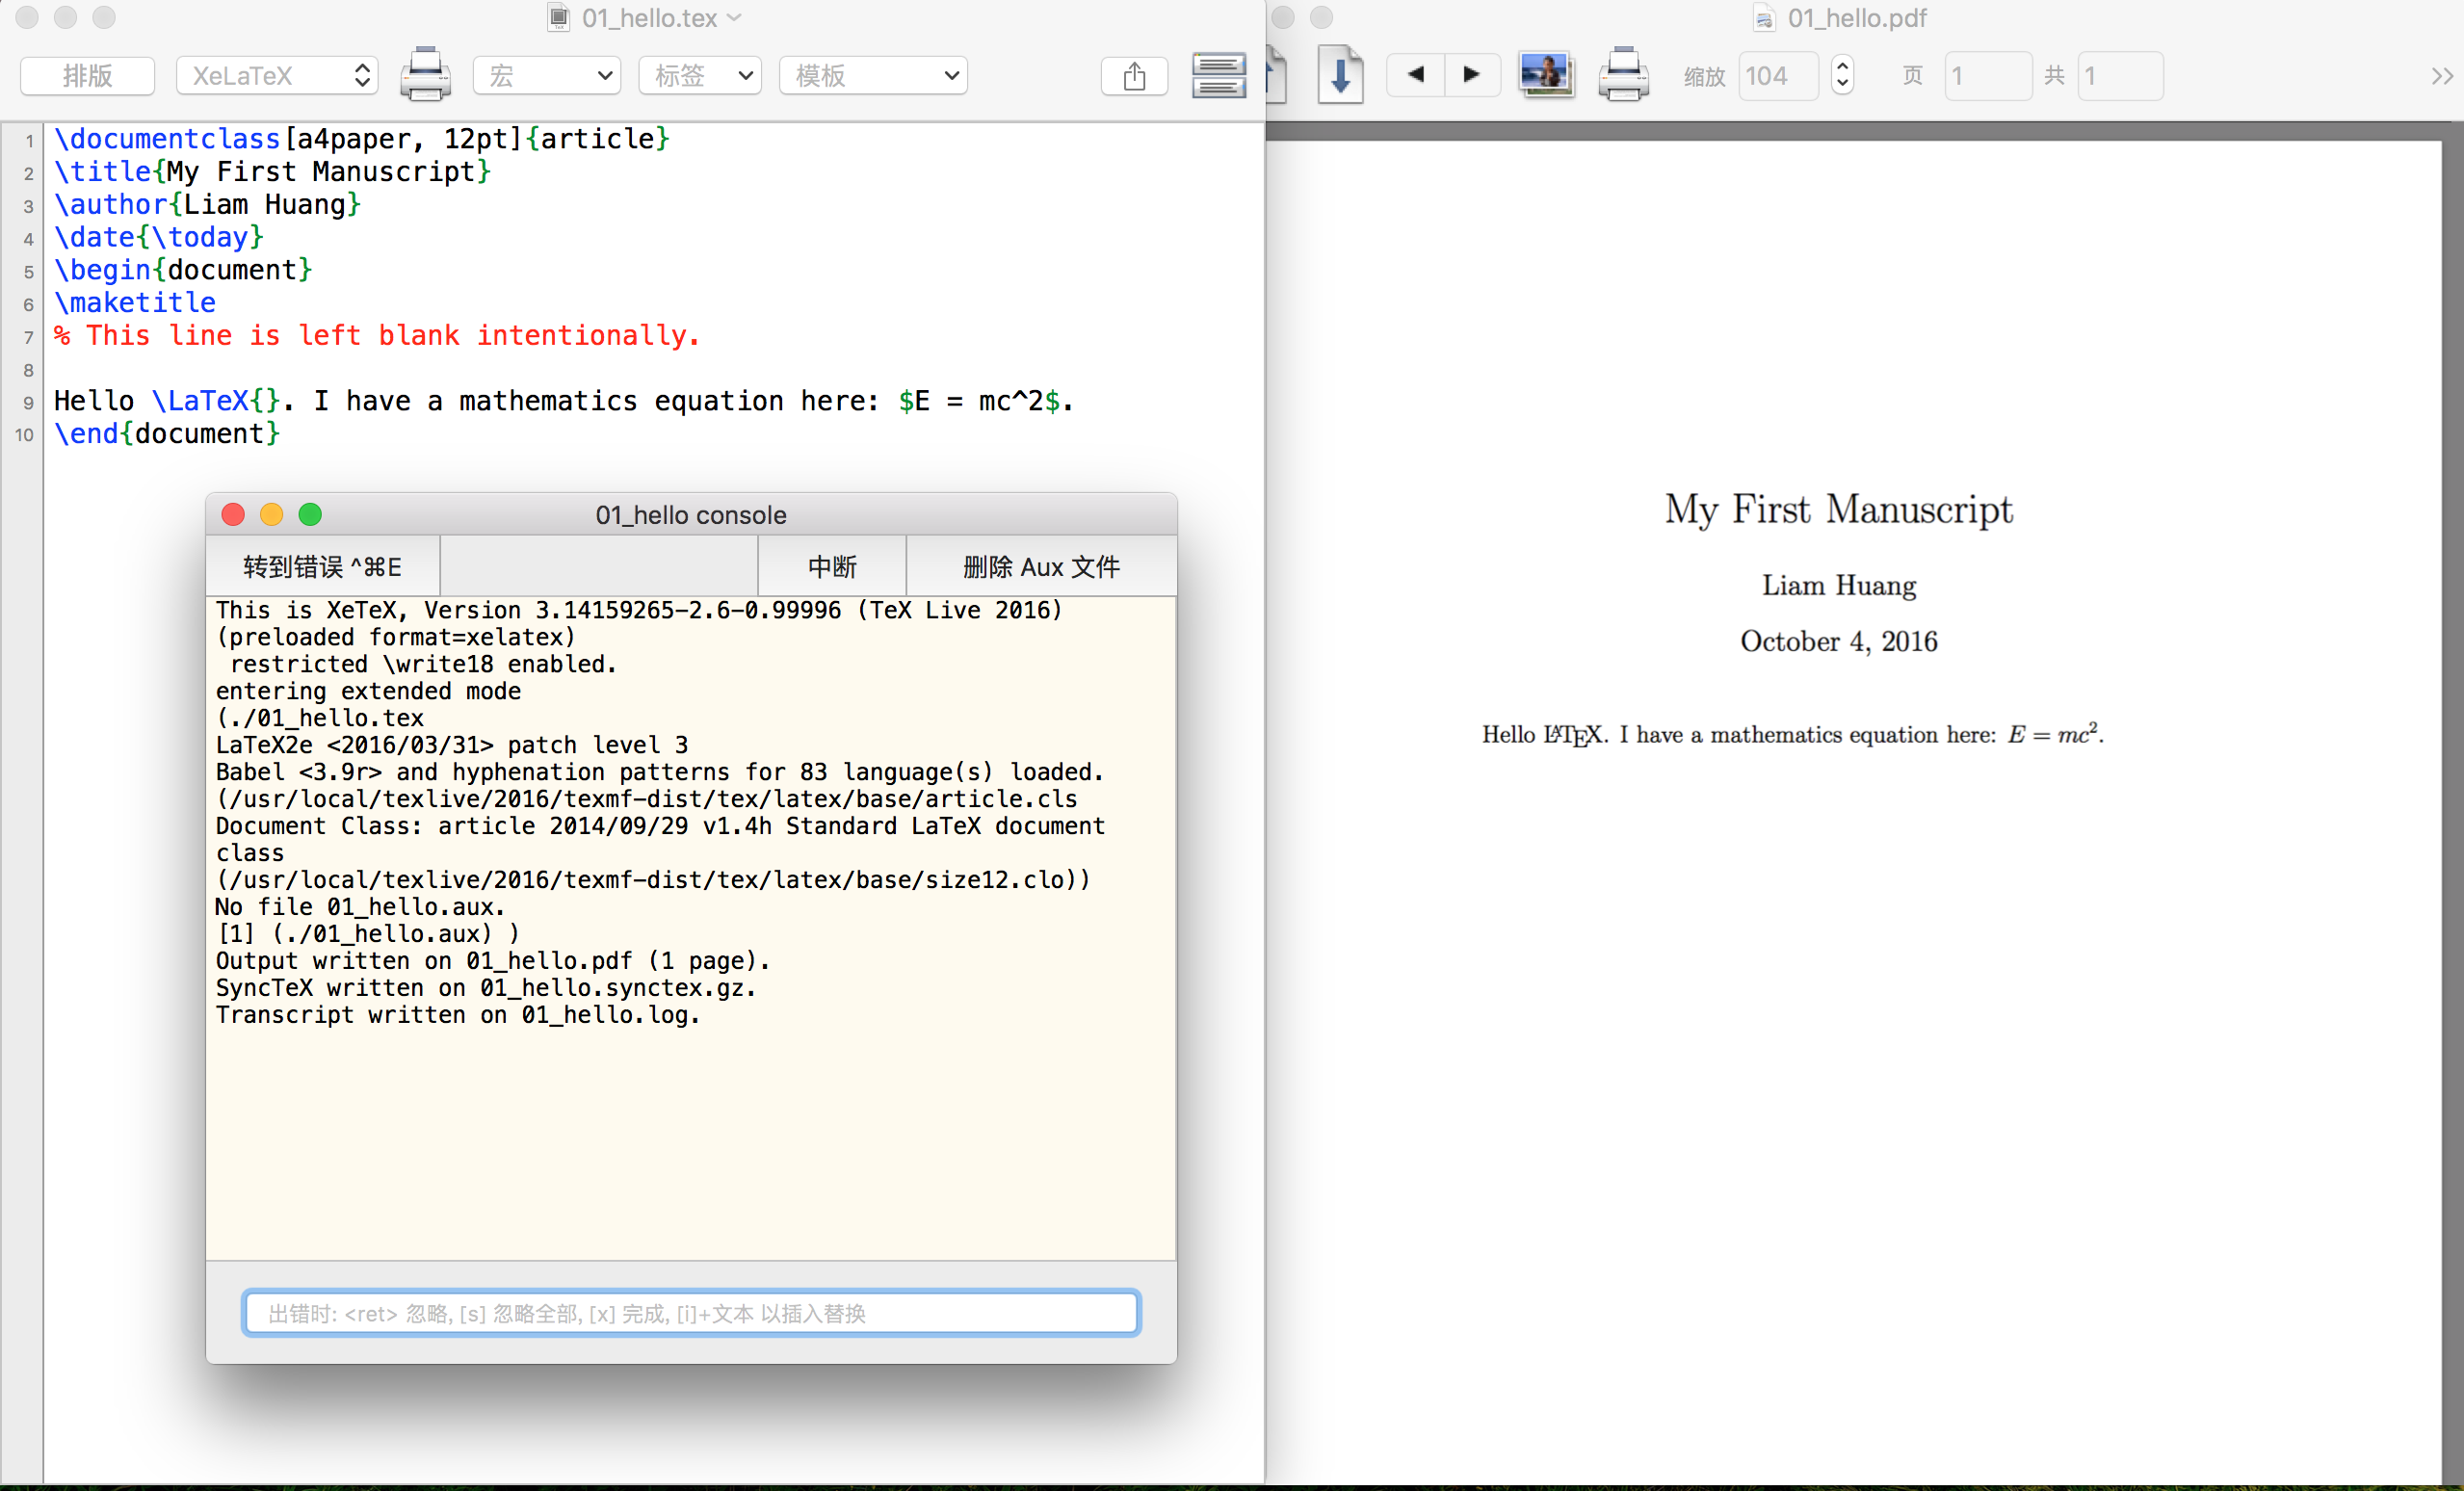
\includegraphics[width = .8\linewidth]{01_hello_mac.png}
\caption{Hello \LaTeX{}}\label{fig:hello}
\end{figure}

如果你看见类似 \ref{lst:hello_wrong} 的输出,这表示你在源代码里写错了一些东西。
请不要慌张,你在学习的过程中会经常遇到类似的问题,最重要的是学会如何阅读错误提示。

\begin{lstlisting}[style = lltx, caption = {错误输出}, label = {lst:hello_wrong}]
! Undefined control sequence.
l.9 Hello \LaTex
                . I have a mathematics equation here: $E = mc^2$.
?
\end{lstlisting}

我们一行一行地看。

\begin{enumerate}
  \item 以一个叹号开头,说明 \LaTeX{} 遇到的错误的名字。这里是「未定义的控制序列」,
  这个错误通常表示你输错了命令,或者使用了一个未经定义的命令。
  \item \lstinline[style = iltx]|l.9| 表示问题出在第九行,
  \lstinline[style = iltx]|Hello \LaTex| 表示 \LaTeX{}
  在处理到这里的时候,遇到了问题。
  \item 第三行是遇到问题时,后续尚未处理的内容。
  \item \LaTeX{} 打印了一个问号,这表示 \LaTeX{} 正在等待我们的输入。
  如果你输入 \lstinline[style = iltx]|x| 则会终止 \LaTeX{} 进程。
\end{enumerate}

这里显而易见,我们将 \lstinline[style = iltx]|\LaTeX| 错误地写作了
\lstinline[style = iltx]|\LaTex|。注意,\LaTeX{} 对命令是区分大小写的。
这里我们将之更正就可以了。

\section{额外习题}

你需要完成这些额外习题,帮助你巩固学到的知识。如果你觉得这部分习题很难,可以先看后面的内容——
但一定要记着回来,解决这些问题。

\begin{enumerate}
  \item 使用搜索引擎(推荐使用 Google),看看 \lstinline[style = iltx]|article|
  文档类还有什么可选参数。修改你的手稿,实际看看这些参数有什么效果。
  \item 删除或者使用 \lstinline[style = iltx]|%| 注释掉
  \lstinline[style = iltx]|\maketitle| 命令,看看会发生什么。思考一下背后的原因。
  \item 尝试打印出更多的内容。
\end{enumerate}

\endinput

% 02_chinese.tex
\chapter{遭遇中文}
\label{chap:chinese}

如果你有认真做第~\ref{chap:hello_world}~章的额外习题,那么你很可能已经发现,
使用 \lstinline[style = iltx]|article| 等\emph{标准文档类}无法在 PDF 文件
中打印中文。今次我们来解决这个问题。

\section{代码和解释}

\begin{lstlisting}[style = lltx, caption = {你好 \LaTeX{}}, label = {lst:chinese}]
\documentclass[UTF8, a4paper, zihao = -4]{ctexart}
\title{第一篇中文手稿}
\author{孟晨}
\date{\today}
\begin{document}
\maketitle
% 这是注释

你好 \LaTeX!我有一个质能方程:$E = mc^2$。
\end{document}
\end{lstlisting}

这份代码和第~\ref{chap:hello_world}~章的代码相似度有 9 分,应该是比较好看懂的。
这里对不同之处做一些解释。

首先是载入文档类的地方,之前载入的是 \lstinline[style = iltx]|article|,
现在载入的是 \lstinline[style = iltx]|ctexart|。这是 \ctex{} 宏集提供的文档类,
用于在 \lstinline[style = iltx]|article| 的基础上提供中文支持和中文版式支持。
与之类似的,还有 \lstinline[style = iltx]|ctexbook| 和
\lstinline[style = iltx]|ctexrep|。它们分别是 \lstinline[style = iltx]|book| 和
\lstinline[style = iltx]|report| 的汉化版。

\lstinline[style = iltx]|ctexart| 是 \lstinline[style = iltx]|article| 的升级版。
因此,\lstinline[style = iltx]|ctexart| 支持 \lstinline[style = iltx]|article| 的
所有参数;并且在 \lstinline[style = iltx]|article| 的基础上有所扩充。
扩充的 \lstinline[style = iltx]|UTF8| 参数,告诉 \ctex{} 宏集,
我们这篇文稿使用 UTF-8 编码。扩充的 \lstinline[style = iltx]|zihao = -4| 参数,
则告诉 \ctex{} 宏集,我们这篇文稿使用小四号字(取代 \lstinline[style = iltx]|12pt|)。

\begin{warning}
  如果没有明确的理由,请不要使用 \pkg{CJK} 宏包。这是一个过时的宏包,并且在中文处理上
  存在很多的问题。

  如果没有明确的理由,也请不要单独使用 \pkg{xeCJK} 宏包。它只解决了中文支持的问题,却没有
  解决中文版式处理的问题。\ctex{} 宏集在使用 \XeLaTeX 时会自动调用 \pkg{xeCJK} 宏包。
\end{warning}

\section{操作和输出}

请将代码清单 \ref{lst:chinese} 中的内容,用键盘逐字母地输入进电脑,
并保存在文件 \file{02\_chinese.tex} 中。注意,请将文件以 UTF-8 编码保存。
点击「排版」,以 \XeLaTeX{} 编译,你应该看到如图 \ref{fig:chinese} 所示的样子。

\begin{figure}[!htb]
\centering
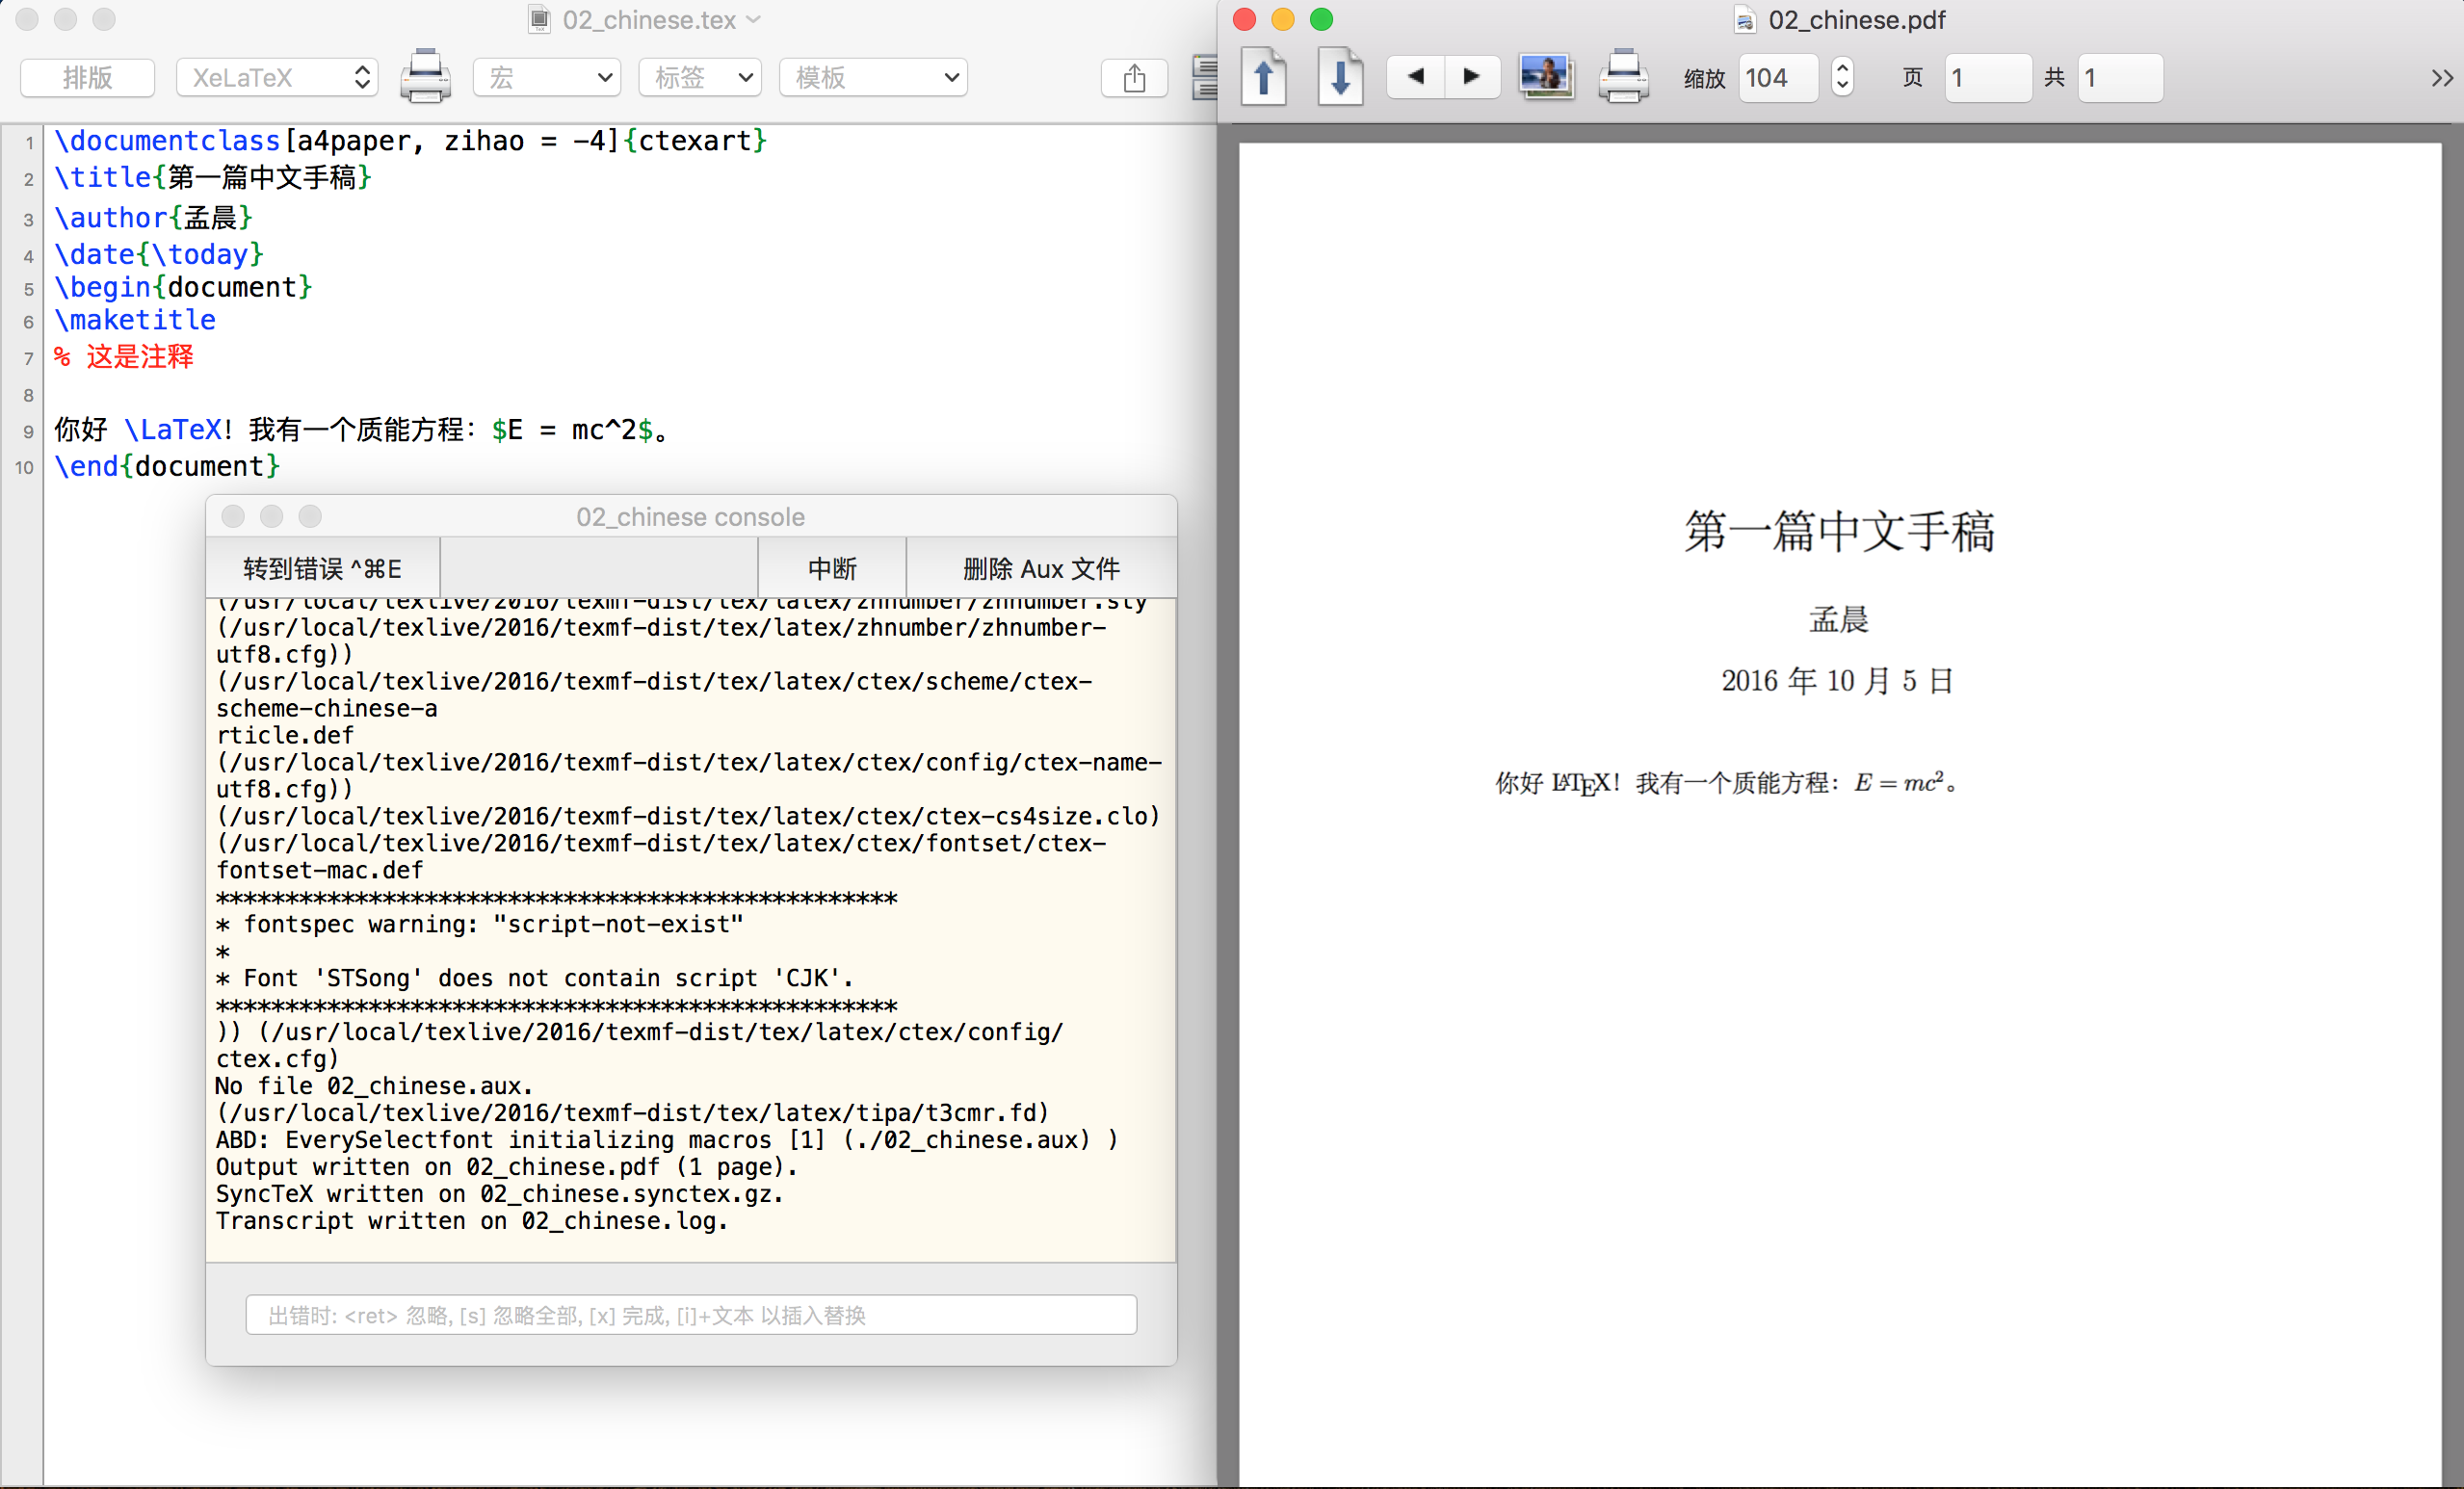
\includegraphics[width = .8\linewidth]{02_chinese_mac.png}
\caption{你好 \LaTeX{}}\label{fig:chinese}
\end{figure}

从此开始,我就不把每次编译的代码、编译窗口和结果一并截图上来了,也不会区分操作系统的版本。
我只会贴出正确的输出结果。
实际上,你应该逐渐养成习惯,明白什么样的代码会打印出什么内容。

\section{额外习题}

你需要完成这些额外习题,帮助你巩固学到的知识。如果你觉得这部分习题很难,可以先看后面的内容——
但一定要记着回来,解决这些问题。

\begin{enumerate}
  \item 使用 \lstinline[style = iltx]|ctexbook| 和
  \lstinline[style = iltx]|ctexrep| 替换 \lstinline[style = iltx]|article|,
  看看会有什么效果。使用搜索引擎,检索相关资料。
  \item 阅读 \ctex{} 宏集的说明书(方法是在命令行中执行
  \lstinline[style = ibash]|texdoc ctex|),了解如果希望%
  \emph{只提供中文支持,不改变版式}应该怎样做。
  \item 尝试打印出这些特殊符号:\#, \$, \textbackslash, \{, \}, \_, \^{}。
  使用搜索引擎,检索\emph{转义符}的相关知识,了解 \LaTeX{} 有哪些符号需要转义才能打印出来。
\end{enumerate}

\endinput

\backmatter

\end{document}
\endinput
